%% ============================================================
%% 分片 18：原文第 6 节「Loop and Line Operators」（原文 glshort.tex 起于第 4483 行）
%% 由 tools/harvmac2tex.py 从 arXiv 源码（hep-th/0604151v3）自动生成。
%% 只译英文散文；公式、编号、\label、\cite 一律不改。
%% ============================================================

\subsection{边界附近的线算子}

\label{sec:lineop}

几何 Langlands 纲领围绕的是这样一种情形：$\Sigma$ 有边界，而线算子平行于该边界。

\begin{figure}[htbp]
\centering
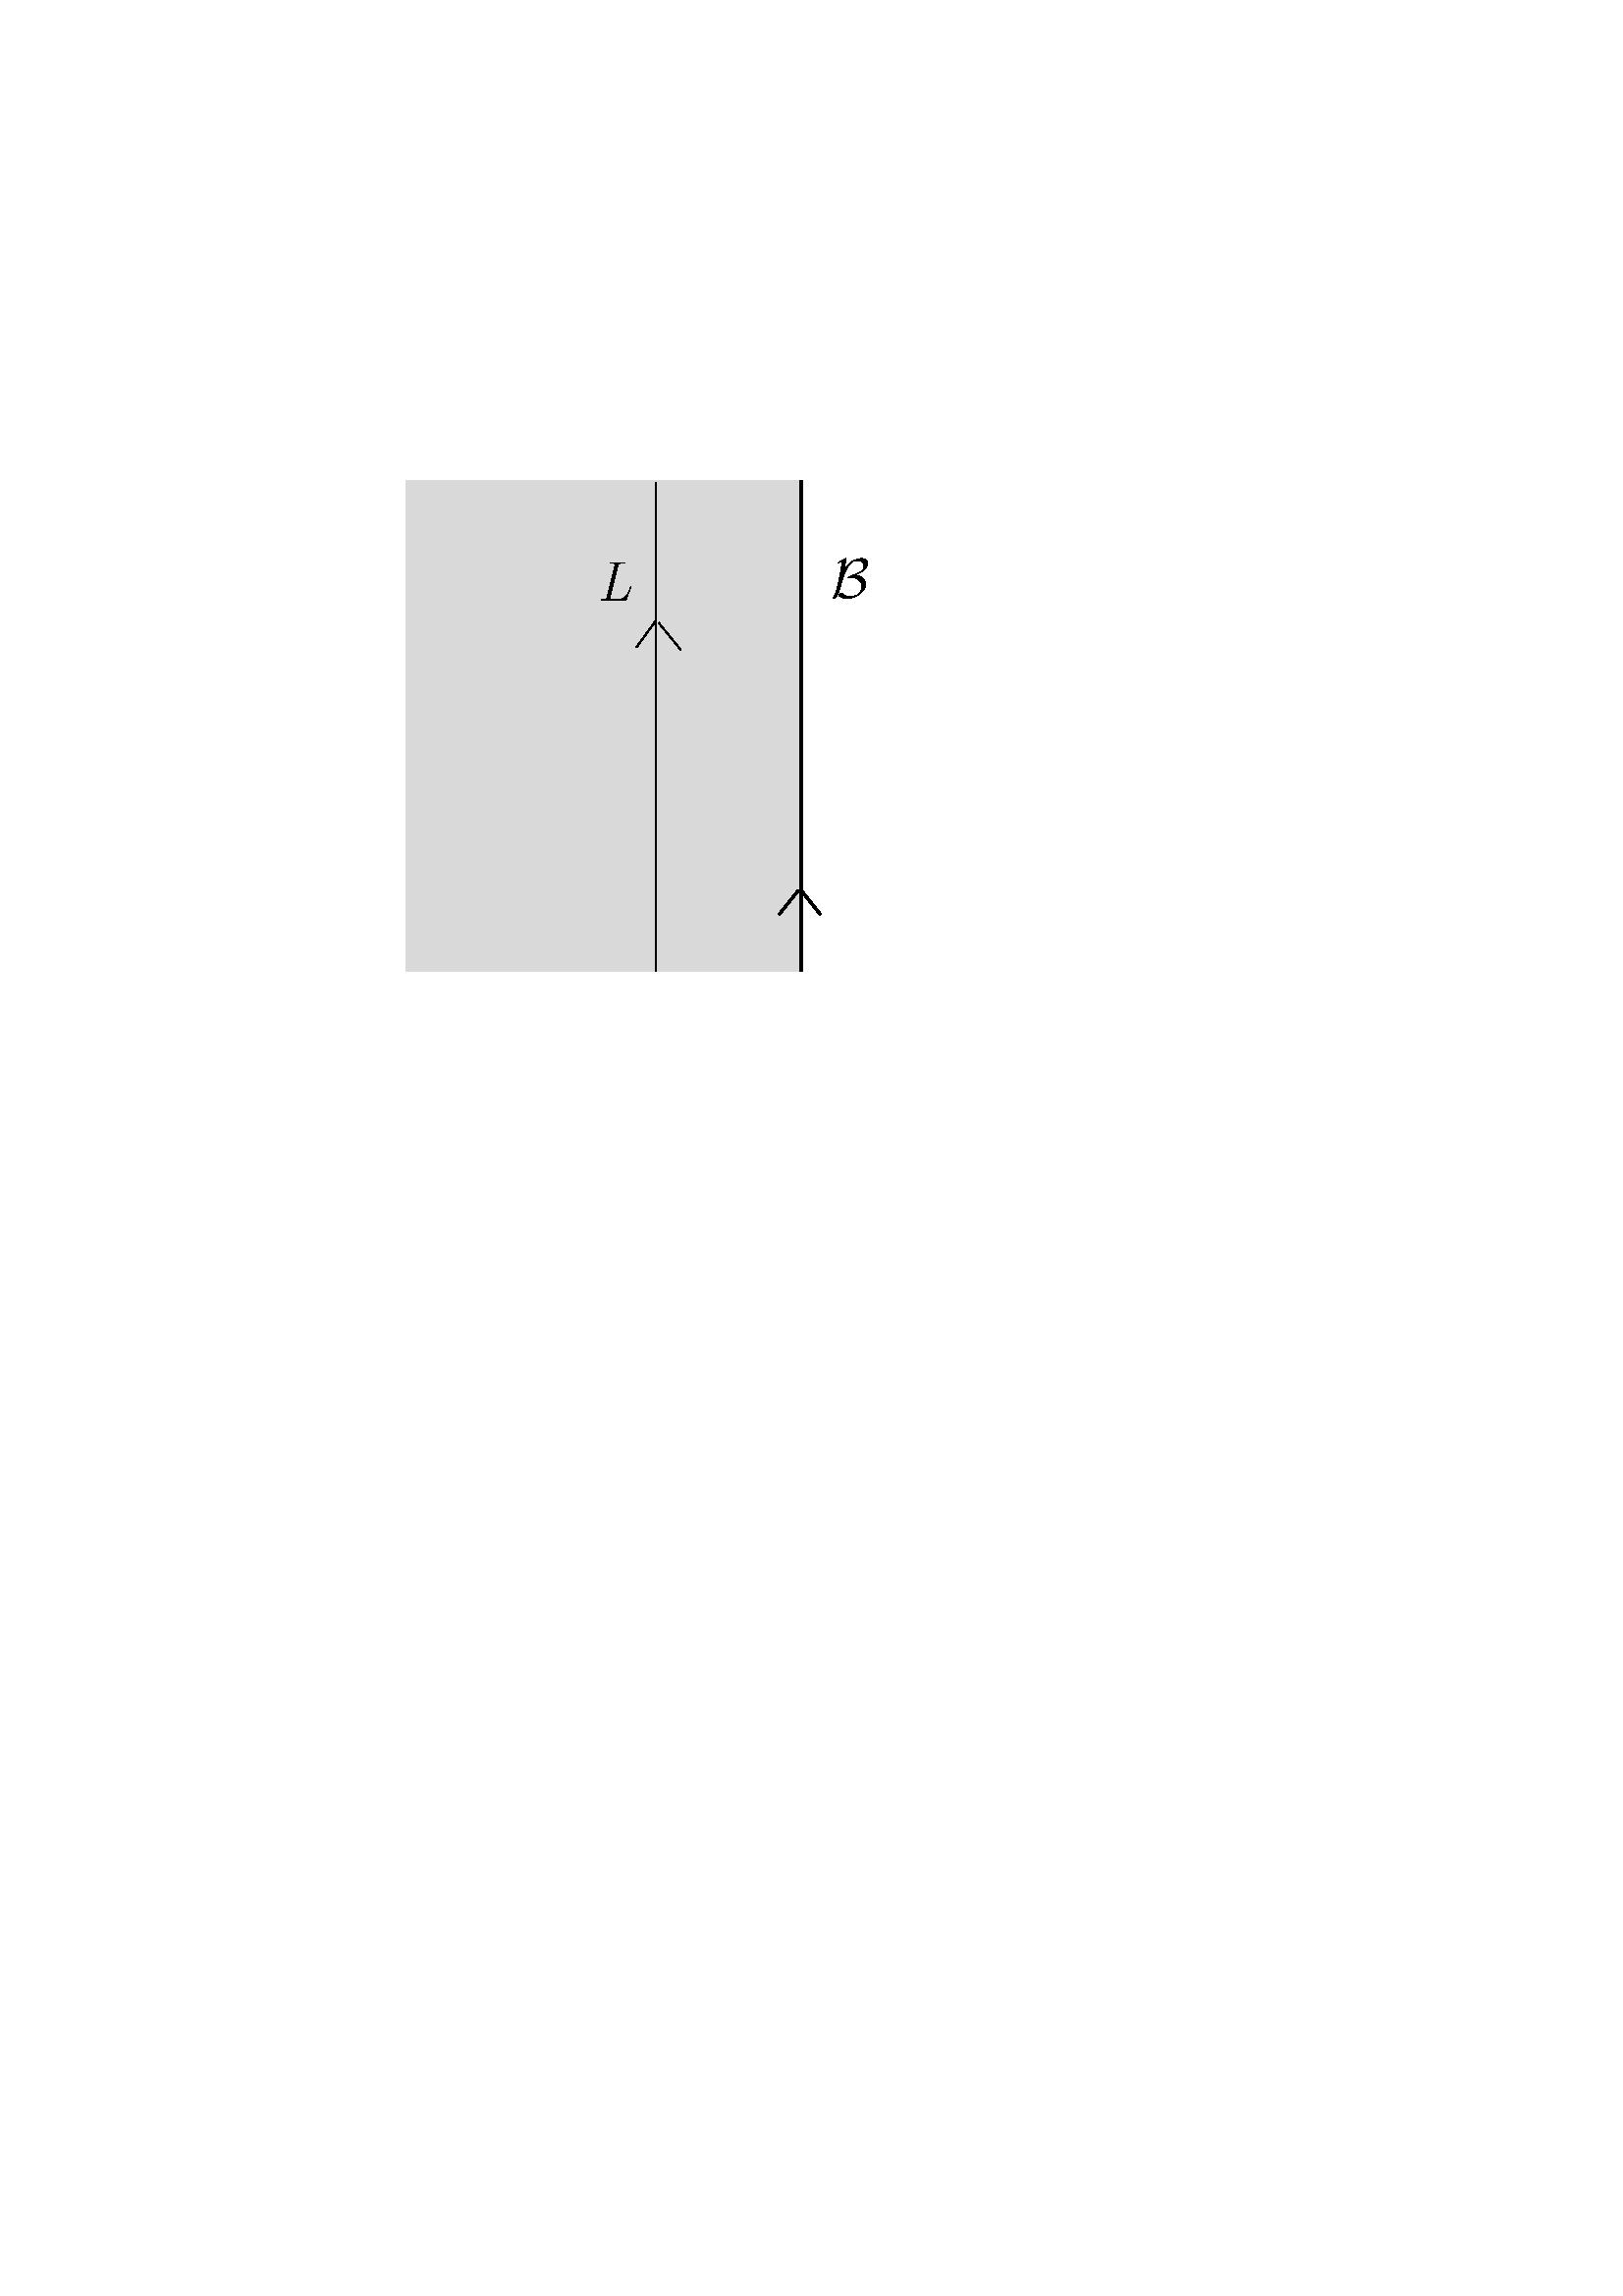
\includegraphics[width=0.75\linewidth]{figures/gla4-4.png}
\caption{带边界的黎曼面，其边界由膜 ${\cal B}$ 标记，另有一条平行于边界的线算子 $L$。（原文 Fig.~7）}
\label{fig:trinamp}
\end{figure}

 在带边界的黎曼面 $\Sigma$ 上定义量子场论需要选定一个边界条件——也就是选定一个膜，我们把它记作 ${\cal B}$。在 \trinamp 中，我们画出一个带边界的黎曼面 $\Sigma$ 以及一条平行于边界的线 $L$。该边界已由膜 ${\cal B}$ 标记，它规定了该边界处的边界条件。线算子 $\EUX$ 支撑在 $L$ 上。$\EUX$ 可以是 Wilson 算子、't Hooft 算子或混合 Wilson-'t Hooft 算子。

{}从宏观观点看，$\EUX$ 与 ${\cal B}$ 只不过合并成一个有效边界条件 ${\cal B}'$。人们可以把 ${\cal B}'$ 刻画为：由于 ${\cal B}$ 与 $\EUX$ 的联合效应，在大距离处看到的那个有效边界条件。或者也可以简单地取 $L$ 趋近边界的极限，让 ${\cal B}'$ 成为所得的极限边界条件。

无论用哪种方式，我们都把由 $\EUX$ 作用于旧膜所产生的新膜记作 ${\cal B}'=\EUX {\cal B}$。这样，我们就把线算子看作作用在边界条件上、产生新边界条件的东西。

\begin{figure}[htbp]
\centering
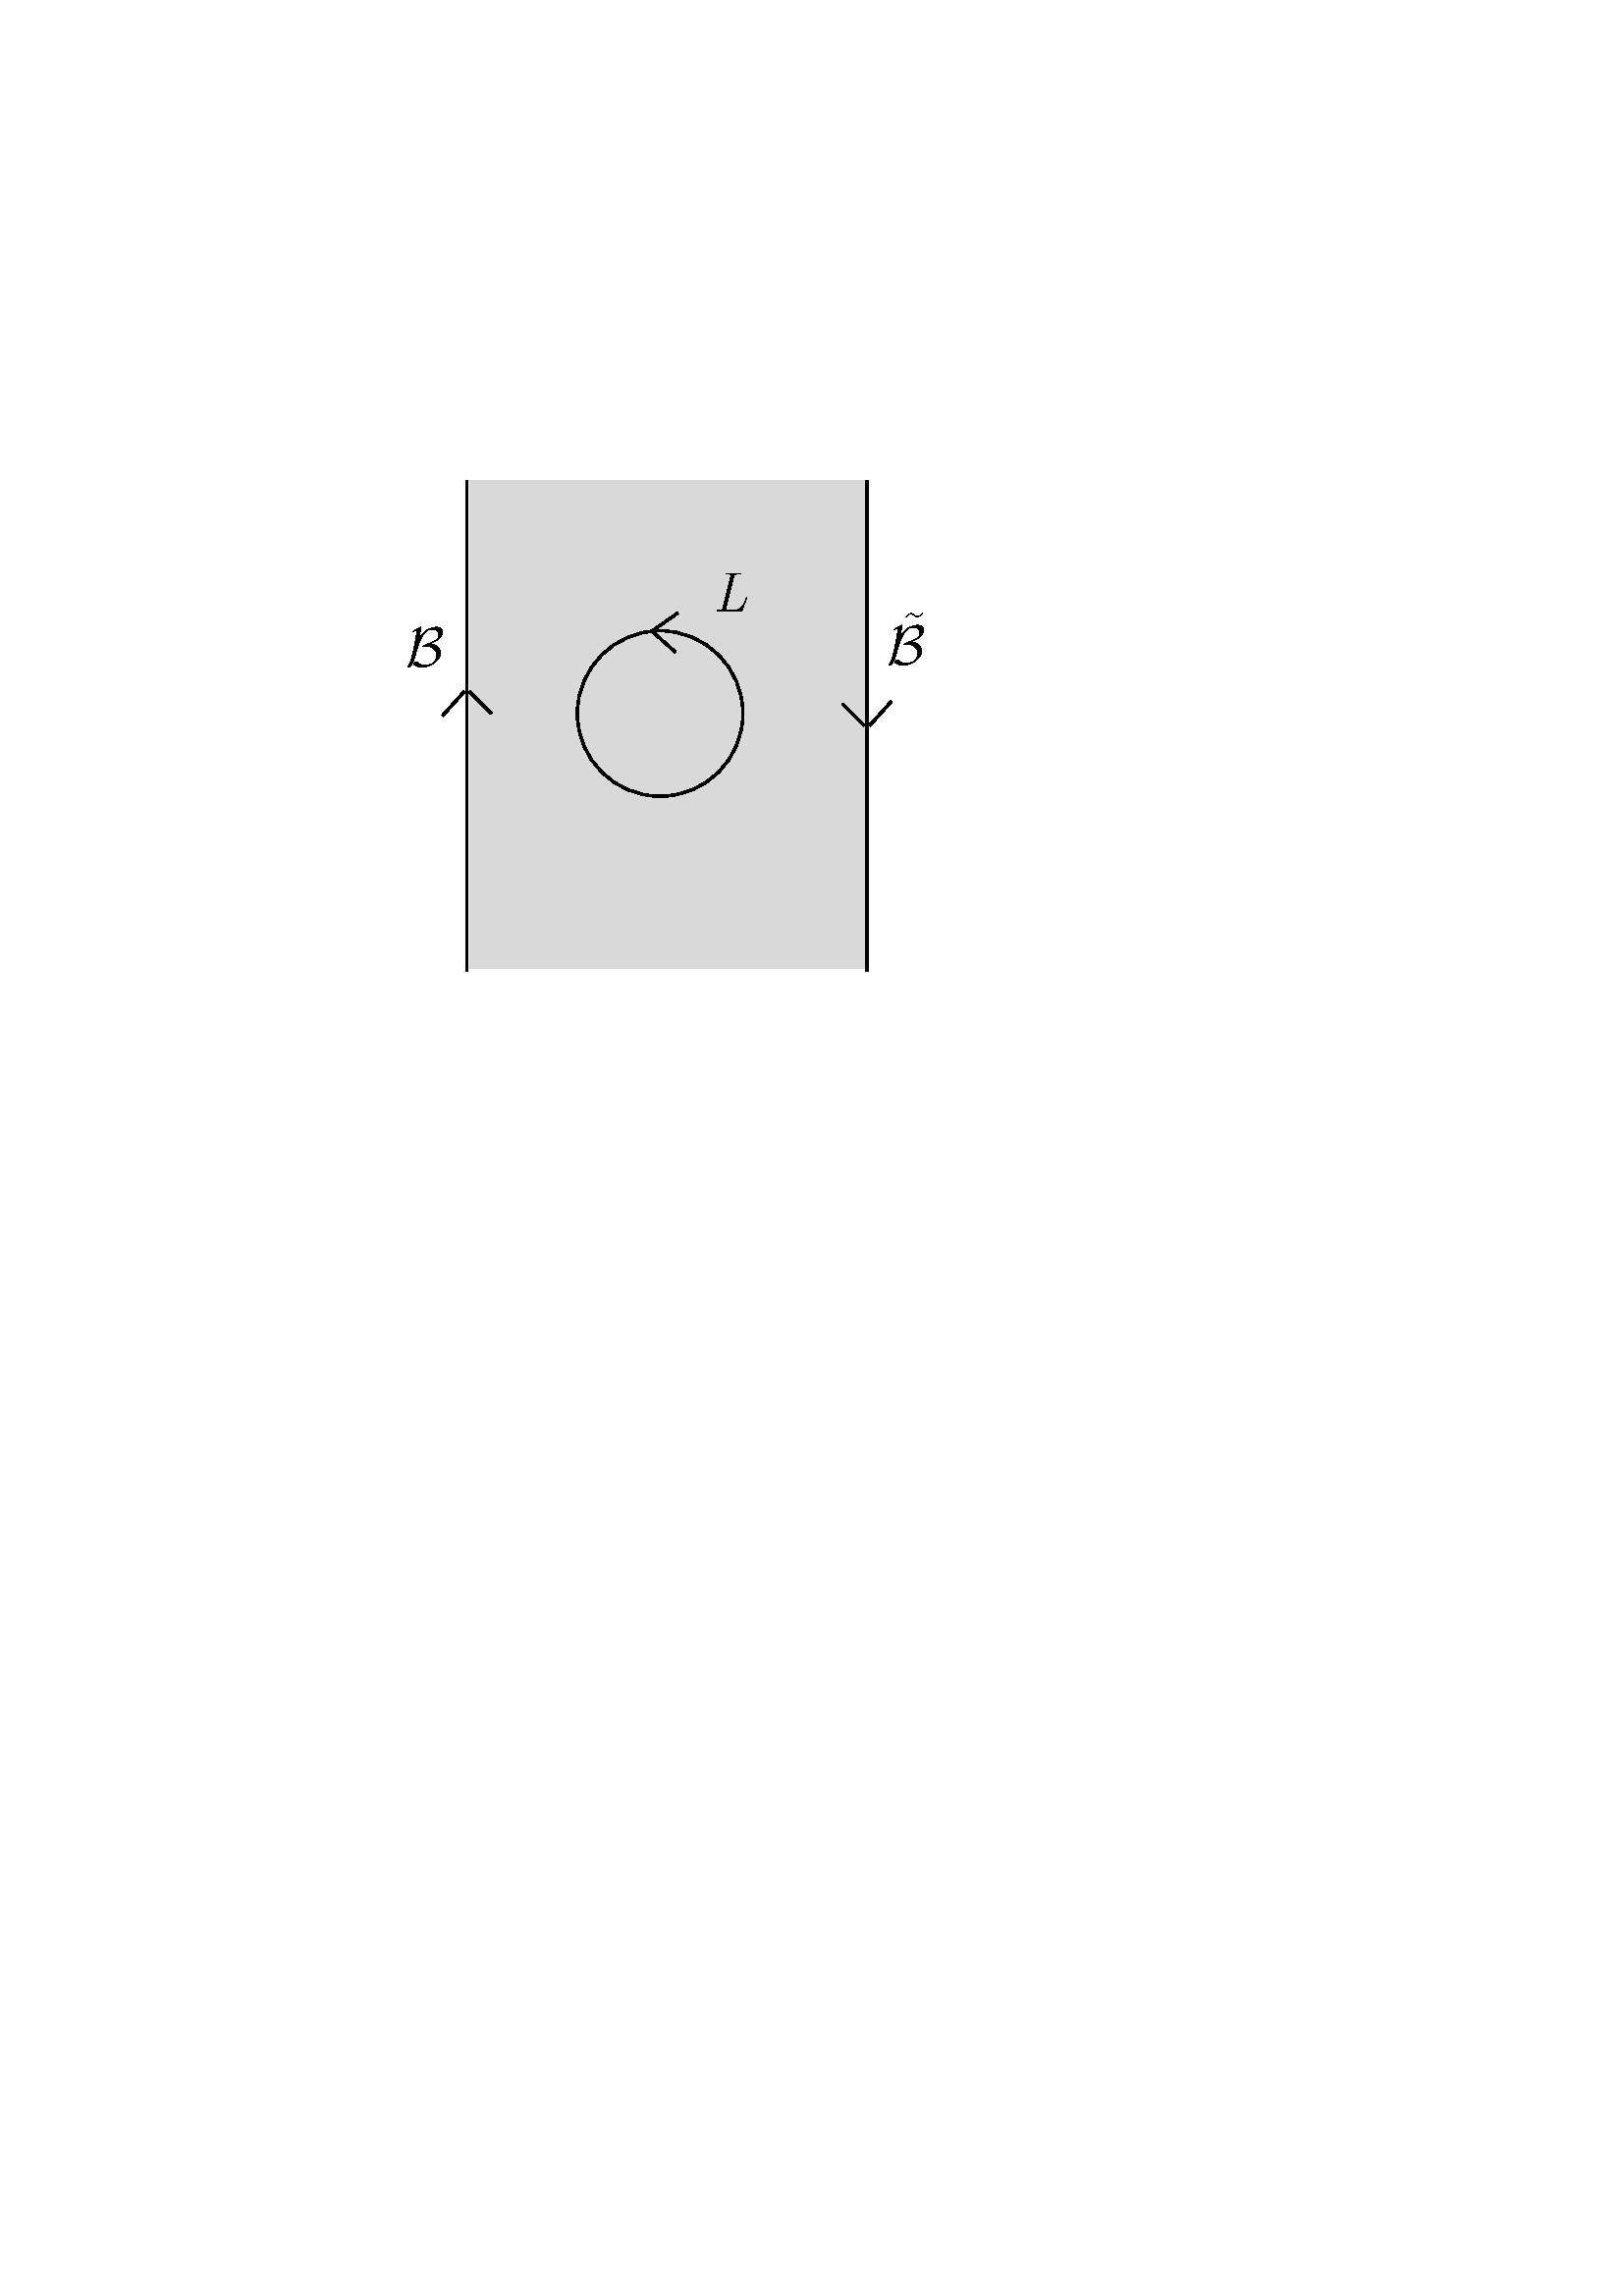
\includegraphics[width=0.75\linewidth]{figures/gla4-5.png}
\caption{圈算子作为普通算子作用在空间 ${\cal H}_{\cal B,\tilde{\cal B}}$ 上。（原文 Fig.~8）}
\label{fig:quadramp}
\end{figure}
 这是一种比算子通常作用于向量空间更为抽象的作用。如我们在上面所见，要得到与 ${\cal B}$ 相联系、可供某个算子作用的向量空间 ${\cal H}_{{\cal B},\tilde
{\cal B}}$，我们需要一对膜 ${\cal B}$ 与 $\tilde {\cal B}$。当然，我们也可以就取 $\tilde {\cal B}={\cal B}$。但即便构造出物理态空间 ${\cal H}_{{\cal B},\tilde {\cal B}}$，真正作用在该空间上的其实是一个{\it 圈}算子——它定域于时间——其作用方式是对 \quadramp 的图景作量子化。而沿时间方向延伸的开线算子（如 \trinamp 中那样）则是另一回事：它是量子化时必须纳入的数据的一部分，只有纳入它才能得到正确的物理态空间。

如果我们{\it 确实}有一个向量空间 ${\cal H}$ 和一个算子 ${\EUO}:{\cal H}\to {\cal H}$，我们就可以寻找 ${\EUO}$ 的本征向量 $\psi\in
{\cal H}$：
% 式 (6.21)
\setcounter{equation}{20}
\begin{equation}\label{eq:reot}
{\EUO}\psi=\lambda\psi.
\end{equation}
 这里 $\lambda$ 是一个普通的复数。

在我们的问题中，不是作用于 Hilbert 空间向量的算子，而是一个更奇异的、经由 ${\cal B}\to {\cal B}'=\EUX {\cal B}$ 作用于理论上的算子。在这种情况下，普通的复本征值没有意义。取而代之，起「本征值」作用的是一个向量空间 $V$。

对每个膜 ${\cal B}$ 与向量空间 $V$，都可定义一个新膜 ${\cal B}\otimes V$。刻画 ${\cal B}\otimes V$ 的一种抽象方式是：对任意膜 $\tilde {\cal B}$，Hilbert 空间 ${\cal H}_{\tilde {\cal B},{\cal B}\otimes V}$ 等于 ${\cal H}_{\tilde {\cal B}, {\cal B}}\otimes V$。

对于由几何构造出的膜，我们可以说得更具体。当理论 $X$ 是靶空间为 $\hat X$ 的二维 sigma 模型时，可以从一个向量丛 ${\cal W}\to \hat X$（或更一般的、可能支撑在子流形上的层）构造出膜。${\cal
W}$ 称为 Chan-Paton 丛。把这样的膜与固定的向量空间 $V$ 作张量积，只不过是把 ${\cal W}$ 换成 ${\cal
W}\otimes V$。当 ${\cal W}$ 换成更一般的层时，这一运算毫无困难地推广。

若把 $V$ 等同于某个 $\Bbb{C}^k$，则把 Chan-Paton 丛与 $V$ 作张量积相当于取原膜的 $k$ 个拷贝。所以 ${\cal B}$ 是 $\EUX$ 的特征膜（eigenbrane）意味着 $\EUX{\cal B}$ 同构于 ${\cal B}$ 的 $k$ 个拷贝的直和。然而，远为更好的做法是把「本征值」想成一个向量空间 $V$，而不只是它的整数维数 $k$，因为 $V$ 实际上可以作为某个参数空间上向量丛的纤维而随附加参数变化。

建立了把膜与向量空间作张量积的概念之后，我们现在就可以定义特征膜的概念。若存在向量空间 $V$ 使得
% 式 (6.22)
\setcounter{equation}{21}
\begin{equation}\label{eq:intico}
\EUX {\cal B}={\cal B}\otimes V,
\end{equation}
 则称膜 ${\cal B}$ 是线算子 $\EUX$ 的特征膜。这一概念对应于 Beilinson 与 Drinfeld 在几何 Langlands 纲领中定义的「特征层」（eigensheaf）概念 \cite{ref5}。

\begin{figure}[htbp]
\centering
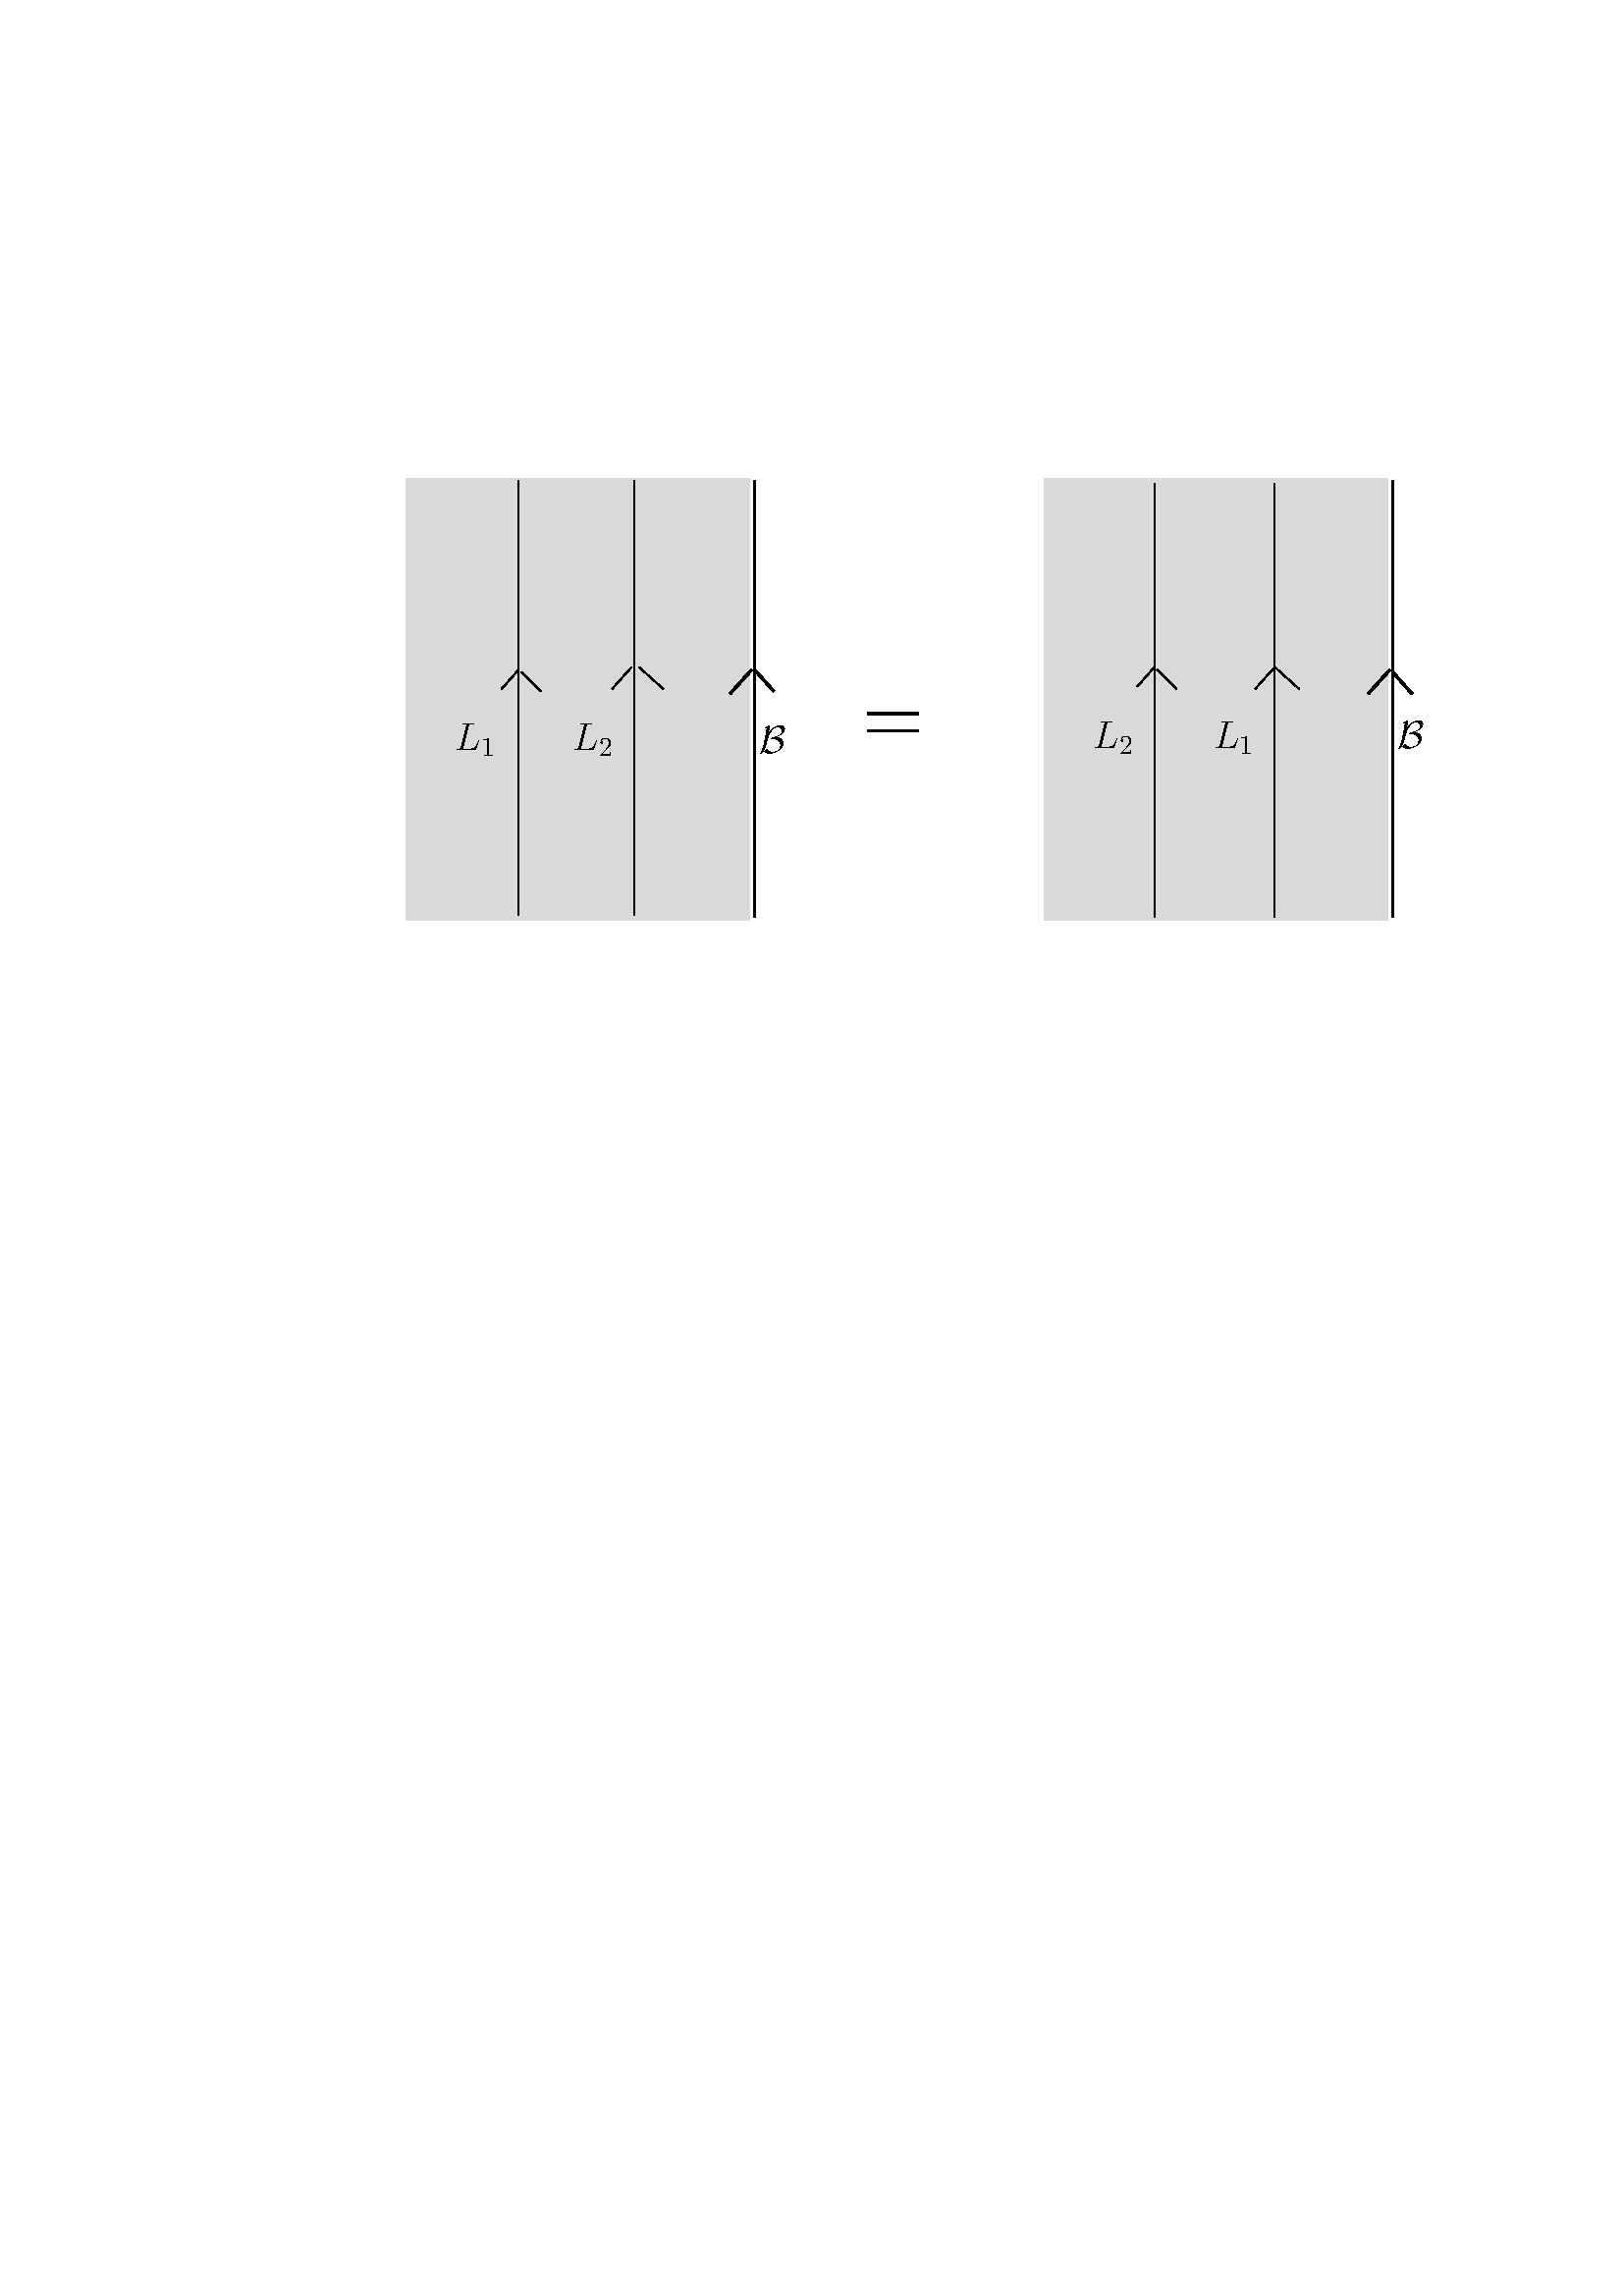
\includegraphics[width=0.75\linewidth]{figures/gla4-6.png}
\caption{若两条线算子 $L_1$ 与 $L_2$ 能彼此穿过而不产生奇异性，则称它们交换。在拓扑场论中，这不过是说此处所画的两幅图可以视为等价。（原文 Fig.~9）}
\label{fig:quintamp}
\end{figure}
 若 $\EUX_1$ 与 $\EUX_2$ 是支撑在平行线 $L_1$ 与 $L_2$ 上的两个线算子，且对所有 ${\cal B}$ 都有
% 式 (6.23)
\setcounter{equation}{22}
\begin{equation}\label{eq:pintico}
\EUX_1\EUX_2{\cal B}=\EUX_2\EUX_1{\cal B}.
\end{equation}
 我们就说它们交换。这一陈述可以用一幅方便的图来说明：它意味着线 $L_1$ 与 $L_2$ 可以彼此穿过而不产生任何不连续性（\quintamp）。正如 Hilbert 空间上的普通算子那样，若两个线算子在此意义下交换，它们就可能具有共同特征膜，即满足下式的膜 ${\cal B}$：
% [WARN] 公式 \eqn\eqref{eq:pintico} 无编号或重复
\begin{equation*}
\tag*{(6.24)}
\begin{aligned}\EUX_1{\cal B}& = {\cal B}\otimes V_1\\
\EUX_2{\cal B}& = {\cal B}\otimes V_2.\\\end{aligned}
\end{equation*}
 更一般地，任意一族交换的线算子都可以有共同特征膜。

\par\medskip{\it 来自四维的线算子}

在我们的问题中，我们关心的是把四维 TQFT 在黎曼面 $C$ 上约化所得的二维 TQFT。此外，我们的线算子全都来自四维的线算子。这就足以保证某些特殊行为。

首先，每个线算子 $\EUX$ 都可以对任意点 $p\in C$ 定义。为明确起见，我们把线算子写成 $\EUX_p$。若保持拓扑对称的膜 ${\cal B}$ 对某个 $p$ 是 $\EUX_p$ 的特征膜，它就必定对每个 $p$ 都是特征膜，因为 $p$ 本来就无关紧要。所以
% 式 (6.25)
\setcounter{equation}{24}
\begin{equation}\label{eq:hintico}
\EUX_p{\cal B}={\cal B}\otimes V_p
\end{equation}
 对某个 $V_p$ 成立。
这里，局部地说，向量空间 $V_p$ 必须与 $p$ 无关，因为 $p$ 无关紧要。但拓扑不变性容许一种可能：当 $p$ 在黎曼面 $C$ 上变化时，$V_p$ 可以有整体单值。所以这些 $V_p$ 是 $C$ 上某个平坦向量丛的纤维。

更明确地说，移动 $p$ 等价于改变 $C$ 上度规的一个特殊情形，而这会把底层作用量改变一个 BRST-平凡的项 $\{Q,\cdot\}$。这一事实使人能够为 $p\in C$ 的向量空间族 $V_p$ 找到一个平坦联络，从而局部地证明 $V_p$ 与 $p$ 无关。但这个平坦联络可以有非平凡的整体单值。

假设给定若干个都保持同一拓扑对称的圈算子 $\EUX_i$。例如，在 $\Psi=\infty$ 处，它们可以是与 $G$ 的表示 $R_i$ 相联系的 Wilson 算子；在 $\Psi=0$ 处，它们可以是与 $^L\negthinspace G$ 的表示 $^L\negthinspace R_i$ 相联系的 't Hooft 算子。无论如何，这些 $\EUX_i$ 都依赖于点 $p_i\in C$。由于我们可以自由地把点 $p_i$ 取为互不相同，我们就可以施行 \quintamp 中的交换——从二维观点看这可能是奇异的——而不遇到任何奇异性。（线算子在四维中并不相交，所以不可能出现奇异性。而且，由于 $C$ 是二维的，移动线算子时有足够的余地，使我们不会遇到沿 $C$ 局部出现的单值。\footnote{若 $L$ 与 $L'$ 是支撑在同一点 $p\in C$ 的两条线算子，要使它们在 $\Sigma\times C$ 中无奇异地彼此穿过，我们把它们分开到两个不同的点 $p,p'\in C$，其中 $p'$ 靠近 $p$。这可以在一个小开球 $U\subset C$ 中做到。对 $\Sigma=\Bbb{R}\times I$，静态线算子支撑在三维流形 $W=I\times C$ 中的点上，而把 $L$ 移过 $L'$ 的操作可以在子空间 $W'=I\times U$ 中完成。$W'$ 中不同点对构成的空间是单连通的，所以在这个局部模型中没有单值，也不存在如何把 $L$ 移过 $L'$ 的歧义。若 $C$ 是一维的，这一论证就不成立。}）因此，具有四维起源的拓扑线算子自动交换。

\par\medskip{\it 电特征膜与磁特征膜}

作为一个特例，$\Psi=\infty$ 处的拓扑 Wilson 算子交换。因此它们可以有共同特征膜。Wilson 线算子的共同特征膜称为电特征膜（electric eigenbrane）。

类似地，$\Psi=0$ 处的拓扑 't Hooft 算子交换，同样可以有共同特征膜。't Hooft 算子的共同特征膜称为磁特征膜（magnetic eigenbrane）。

$S$-变换 $S:\Psi\to -1/n_{\frak g}\Psi$ 把拓扑 Wilson 算子映为拓扑 't Hooft 算子，从而把电特征膜映为磁特征膜。

与任何一族来自四维的线算子的特征膜一样，电特征膜与磁特征膜自动与 $C$ 上的平坦向量丛相联系。这是几何 Langlands 纲领中的一个重要陈述。如我们所见，它反映了二维以上存在一个底层的 TQFT。

\par\medskip{\it 交换线算子的代数}

来自四维的线算子交换这一事实引出了另一个问题：它们生成的是什么交换代数？

在 Wilson 线算子的情形，它就是 $G$ 的表示的张量代数。换句话说，设 $R$ 与 $\tilde R$ 是 $G$ 的两个表示，并设 $R\otimes \tilde R$ 按不可约表示的分解为 % 式 (6.26)
\setcounter{equation}{25}
\begin{equation}\label{eq:ico}
R\otimes \tilde R=\oplus_\alpha n_\alpha R_\alpha.
\end{equation}

这里我们取 $R_\alpha$ 为{\it 互不相同}的不可约表示；整数 $n_\alpha$ 是 $R_\alpha$ 在 $R\otimes \tilde R$ 的分解中出现的重数。（关系 \eqref{eq:ico}\ 以及下面的其它关系，都可以用维数为 $n_\alpha$ 的向量空间 $N_\alpha$ 更精确地表述，但我们把这个精化推迟到第~\ref{sec:opprod}~节。）

我们考虑平行线 $L$ 与 $L'$，并考虑 $L$ 趋近 $L'$ 的极限。我们断言 % 式 (6.27)
\setcounter{equation}{26}
\begin{equation}\label{eq:tryo}
\lim_{L\to
L'}W(R,L)\cdot W(\tilde R,L')=\sum_\alpha n_\alpha W(R_\alpha,L').
\end{equation}
 事实上，由于超对称，该极限可以经典地计算。若我们考虑的是普通的 Wilson 算子而非超对称的 Wilson 算子，则在 $L\to L'$ 的极限中会有各种量子效应。在超对称情形，我们可以直接令 $L=L'$ 并作经典计算。

有了这一点，计算便一路顺风。对闭圈而言，$W(R)$ 与 $W({\tilde R})$ 分别是表示 $R$ 与 $\tilde R$ 中的和乐。它们的乘积是表示 $R\otimes \tilde R$ 中的和乐；而由 \eqref{eq:ico}，它可以展开为表示 $R_\alpha$ 中和乐之和，从而给出 \eqref{eq:tryo}。对线算子而言，$W(R)$ 或 $W(\tilde R)$ 通过平行移动作用在 $R$ 或 $\tilde R$ 表示中的初态上，而这些初态的张量积具有如 \eqref{eq:tryo} 那样的直和分解。

更不正式地说，Wilson 算子 $W(R)$ 与 $W(\tilde R)$ 描述表示 $R$ 与 $\tilde R$ 中的外电荷。它们的乘积描述表示 $R\otimes\tilde R$ 中的一对电荷，其按不可约表示的分解给出超对称 Wilson 算子的 OPE。

对偶地，我们预期：若 $^L\negthinspace R$ 与 $^L\negthinspace{\tilde R}$ 是 $^L\negthinspace G$ 的表示，且 % 式 (6.28)
\setcounter{equation}{27}
\begin{equation}\label{eq:itro}
^L\negthinspace R\otimes{}
^L\negthinspace\tilde R=\oplus_\alpha n_\alpha\, {}^L\negthinspace R_\alpha,
\end{equation}

则 % 式 (6.29)
\setcounter{equation}{28}
\begin{equation}\label{eq:hffo}
\lim_{L\to L'}T({}^L\negthinspace
R,L)T({}^L\negthinspace\tilde R,L')=\sum_\alpha n_\alpha T({}^L\negthinspace
R_\alpha,L').
\end{equation}


对某些群与表示，例如在 \cite{ref86,ref87} 所研究的情形，规范理论与弦之间的对偶使这一结果变得清楚。但在物理学文献中，我们不知道有任何尝试直接在规范理论中计算 't Hooft 算子的算子乘积展开。在第~\ref{sec:thooftheckeop}~节中，我们将建立 't Hooft 算子与 Hecke 变换之间的关系，然后在第~\ref{sec:opprod}~节中我们将看到 \eqref{eq:hffo}\ 这一陈述如何与数学文献中所知的结果相关 \cite{ref97,ref98}。

我们可以通过在 Coulomb 分支上研究 't Hooft 算子的算子乘积展开来获得 \eqref{eq:hffo} 中系数的一些信息；在 Coulomb 分支上，规范群破缺到一个阿贝尔子群。给定两个 't Hooft 算子 $T({}^L\negthinspace R,L)$ 与 $T({}^L\negthinspace  R',L')$，设 $^L\negthinspace w$ 与 $^L\negthinspace w'$ 分别是两个表示 $^L\negthinspace R $ 与 $^L\negthinspace R'$ 的最高权。在 Coulomb 分支上，这些 't Hooft 算子通过奇异单极子解起作用，其磁荷是 $^L\negthinspace G$ 的权 $^L\tilde w$ 与 $^L\tilde w'$；这里 $^L\tilde w$ 与 $^L\tilde w'$ 可以是 $^L\negthinspace w$ 与 $^L\negthinspace w'$ 的任意 Weyl 变换。两个 't Hooft 算子的乘积由一个磁荷为 $^L\tilde w+{}^L\tilde w'$ 的奇异阿贝尔单极子表示。为使表示 $^L\negthinspace R_i$ 出现在算子乘积展开 \eqref{eq:hffo} 中，其最高权 $^L\negthinspace w_i$ 必须等于 $^L\tilde w+{}^L\tilde w'$，其中 $^L\tilde w$ 与 ${}^L\tilde w'$ 取某种选择。无论我们怎样选择 $^L\tilde w$ 与 $^L\tilde w'$，它们的和 $^L\hat w={}^L\tilde w+{}^L\tilde w'$ 都被 $^L\bar w={}^L\negthinspace w+{}^L\negthinspace w'$ 支配（意思是 $^L\bar w -{}^L\hat w$ 是支配权，可以为零）。$^L\negthinspace R_i$ 的一种可能是：它可以是最高权恰为 $^L\bar w$ 的那个表示 $^L\negthinspace\bar R$。这个表示在展开 \eqref{eq:hffo}\ 中以恰好 $n=1$ 的重数出现，因为使 $^L\tilde w$ 与 $^L\tilde w'$ 之和等于 $^L\bar w$ 的选择恰有一种。其它可能出现的表示，是其最高权被 $^L\bar w$ 支配的那些表示。我们把它们称为 $^L\negthinspace\bar R$ 的相伴表示（associated representations）。对于这些次支配的或相伴的表示，没有直接的办法推出算子乘积展开中的系数。最终我们会在第~\ref{sec:opprod}~节看到，它们来自 Hecke 修改空间的奇异性，这就解释了为什么确定它们很微妙。

\par\medskip{\it 作用在膜范畴上的函子}

到目前为止我们所说的，还没有完全把握住线算子在二维中的形式性质。

我们已经说明，保持适当拓扑对称的线算子 $\EUX$ 在膜上有自然的作用。若 ${\cal B}$ 与 ${\cal B}'$ 是任意两个膜，我们可以用 $\EUX$ 作用在它们上，得到新膜 $\EUX{\cal B}$ 与 $\EUX{\cal B}'$。与这对膜 ${\cal B}$ 和 ${\cal B}'$ 相联系的是一个物理态空间 ${\cal H}_{{\cal
B},{\cal B}'}$，它由量子化 $({\cal B},{\cal B}')$ 开弦得到。同样，与这对膜 $\EUX{\cal B}$ 和 $\EUX{\cal B}'$ 相联系的是物理的 $(\EUX{\cal B},\EUX{\cal
B}')$ 弦的空间 ${\cal H}_{\EUX
{\cal B},\EUX{\cal B}'}$。

\begin{figure}[htbp]
\centering
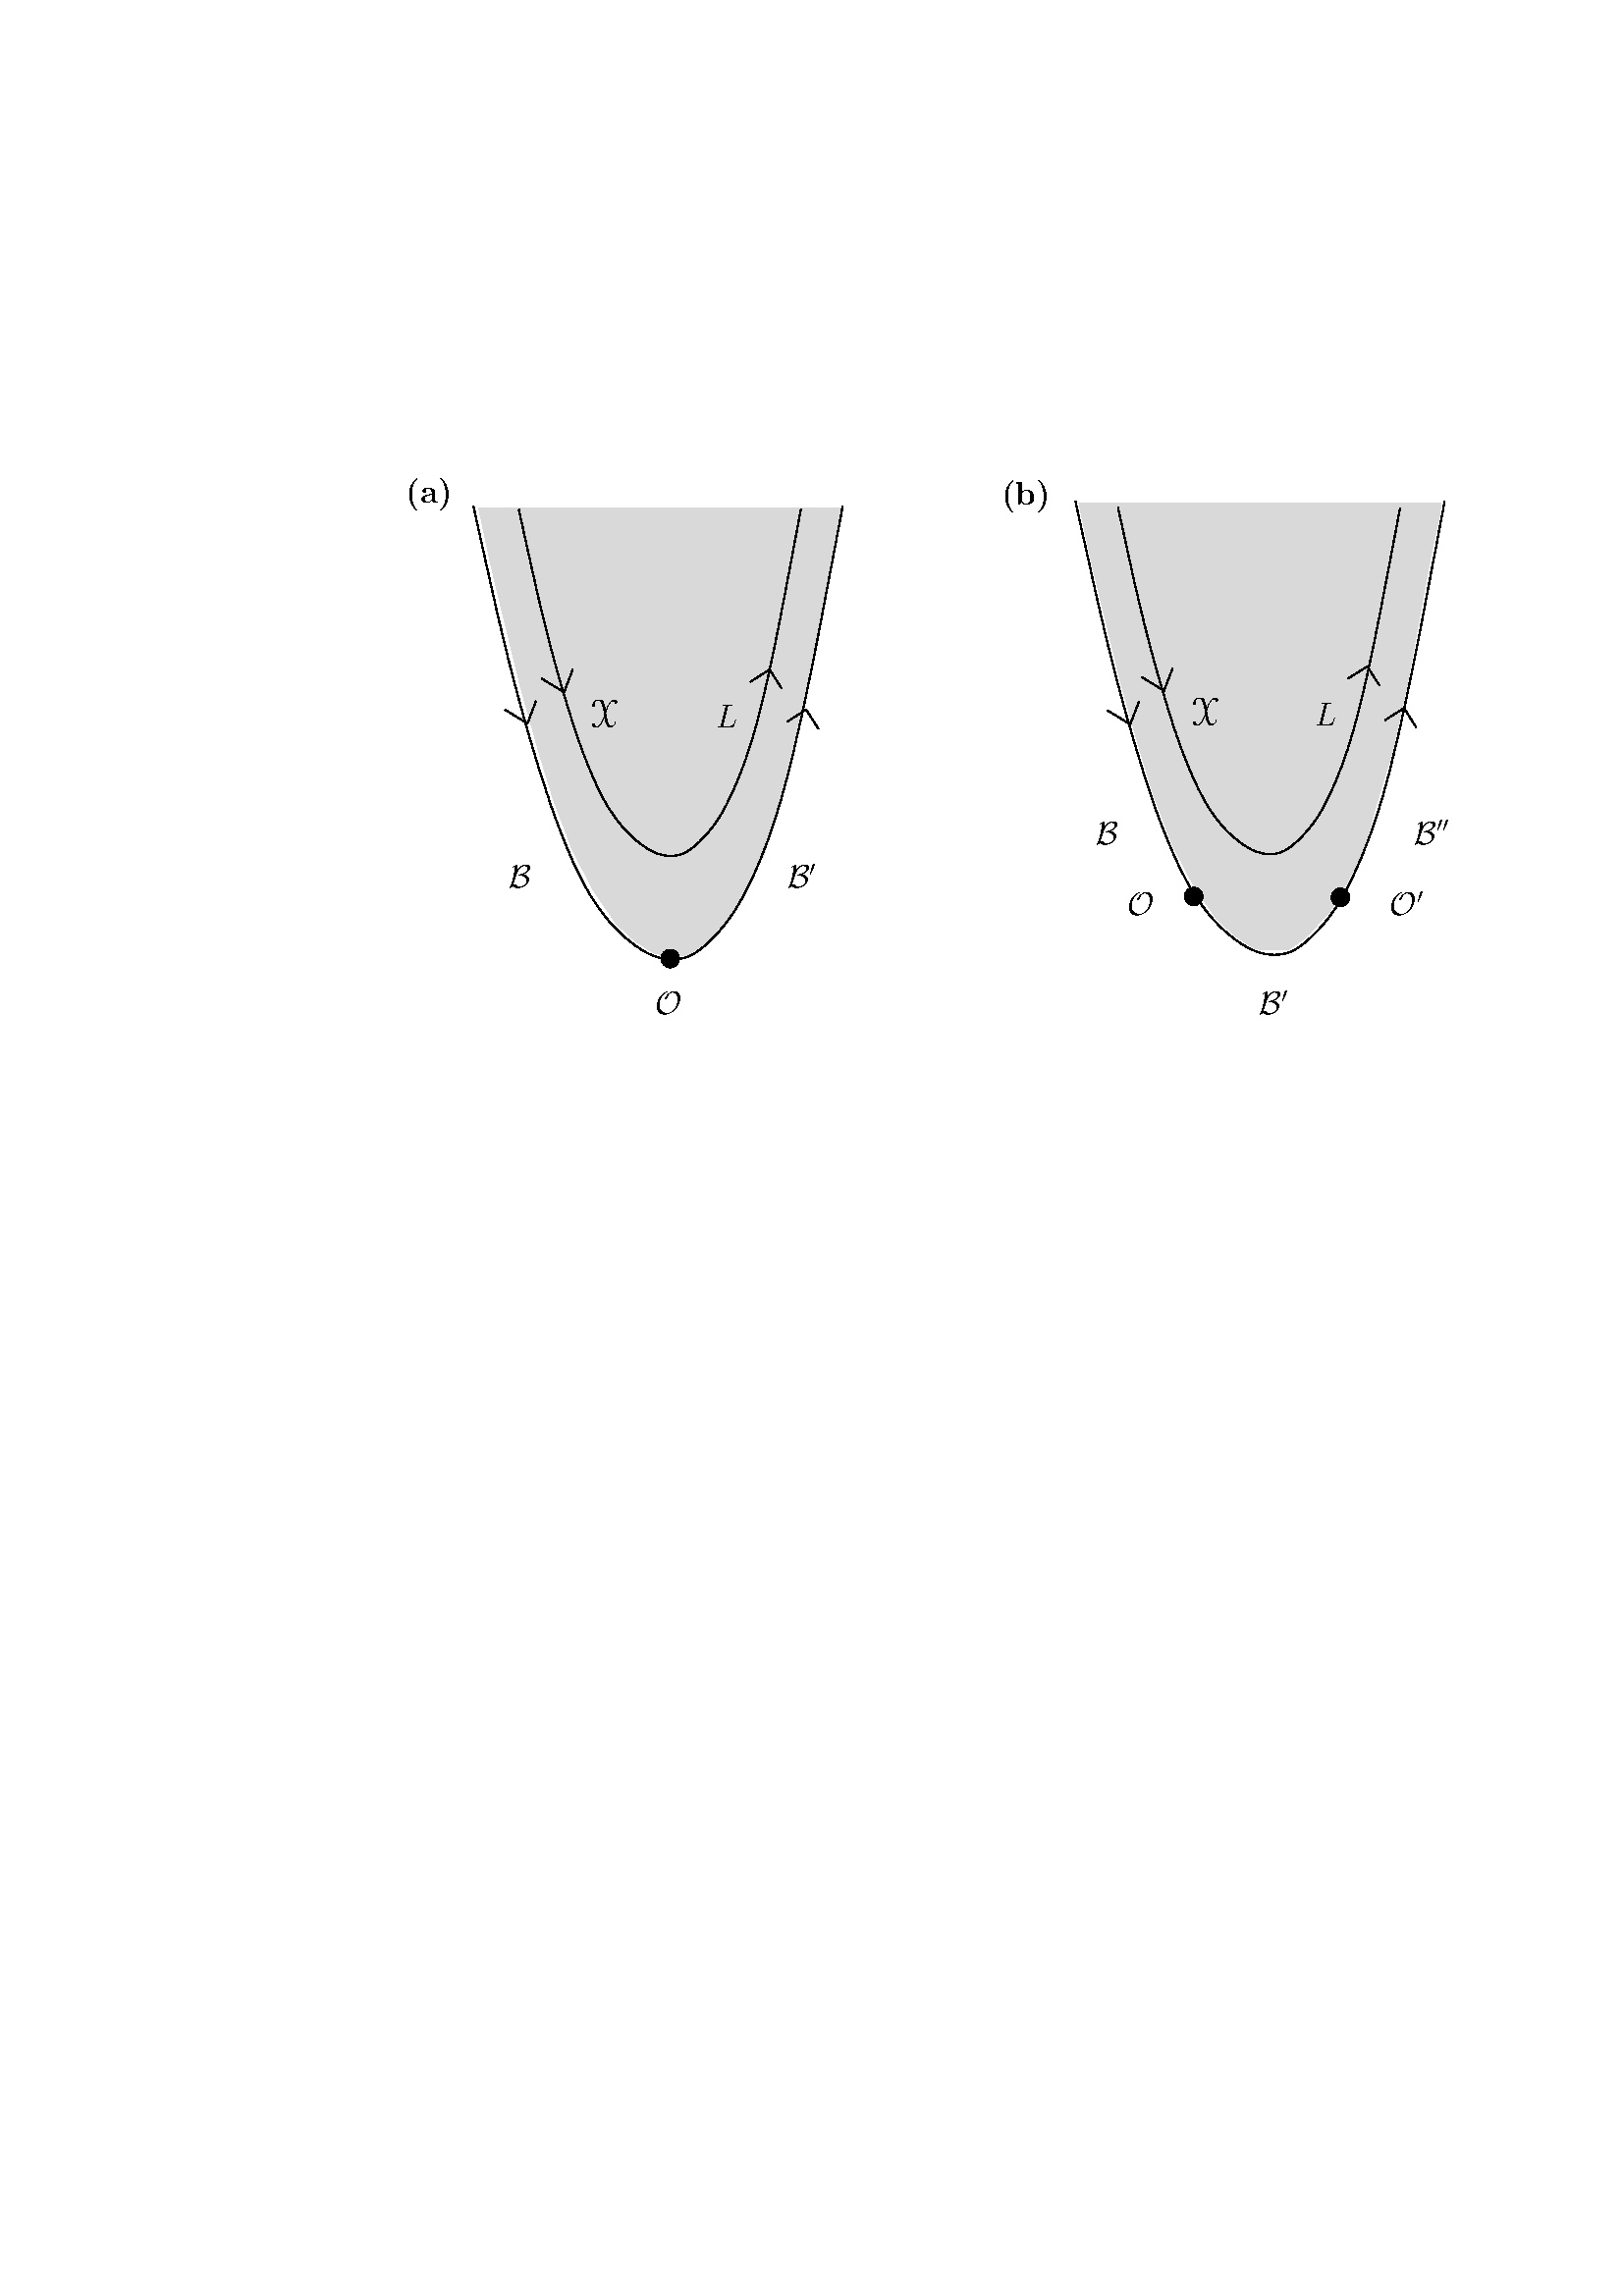
\includegraphics[width=0.75\linewidth]{figures/gla4-6-5.png}
\caption{(a) 支撑在线 $L$ 上的线算子 $\EUX$ 把膜 ${\cal B}$ 与 ${\cal B}'$ 映为膜 $\EUX{\cal B}$ 与 $\EUX{\cal B}'$，同样把 $({\cal B},{\cal B}')$ 弦映为 $(\EUX{\cal B},\EUX{\cal B}')$ 弦。图中算子 ${\EUO}$ 确定一条 $({\cal B},{\cal B}')$ 弦，它被线算子映为一条 $(\EUX{\cal B},\EUX{\cal B}')$ 弦。(b) 这些映射保持开弦乘法的结合律。（原文 Fig.~10）}
\label{fig:zingop}
\end{figure}
 与线算子 $\EUX$ 相联系的是一个自然映射 $\hat\EUX:{\cal H}_{{\cal
B},{\cal B}'}\to{\cal H}_{\EUX{\cal B},\EUX{\cal B}'}$。$\hat \EUX$ 的定义从 \zingop(a) 应当很清楚。在那幅图中，从微观观点看，算子 ${\EUO}$ 确定 ${\cal H}_{{\cal B},{\cal B}'}$ 中的一个态；但从宏观观点看，当 $L$ 趋近边界时，我们看到的是 ${\cal H}_{\EUX{\cal
B},\EUX{\cal B}'}$ 中的一个态。

恰当地说，若 ${\EUO}$ 是恒等算子的倍数，则边界上不存在 ${\EUO}$ 被插入的特殊点，而在线算子 $\EUX$ 趋近边界之前或之后这都是对的。所以 $\hat\EUX$ 把 ${\cal H}_{{\cal B},{\cal B}}$ 中的恒等元（即对应于恒等算子 ${\EUO}=1$ 的开弦态）映为 ${\cal H}_{\EUX{\cal B},\EUX{\cal B}}$ 中的恒等元。它还保持开弦的乘法。事实上，给定三个膜 ${\cal B}$、${\cal B}'$ 与 ${\cal B}''$，结合乘法 ${\cal H}_{{\cal B},{\cal B}'}\otimes{\cal
H}_{{\cal B}',{\cal B}''}\to {\cal H}_{{\cal B},{\cal B}''}$ 是由如 \dunamp(b) 那样粘接开弦定义的，或者等价地由边界上插入算子的算子乘积展开定义，如 \zingop(b) 所示。这显然与把线算子移到边界处的操作交换。概括这些陈述的漂亮说法是：线算子 $\EUX$ 确定了一个把膜范畴映到自身的函子。

把线算子看作膜范畴的对称性，在 \cite{ref99} 中已从不同的观点独立讨论过。它们与对偶变换的关系将在别处讨论 \cite{ref26}。关于用类 Wilson 算子描述二维共形场论中边界微扰的例子，见 \cite{ref100} 的第 5.5 节。

\par\medskip{\it 线算子与增强超对称}

特殊的 Wilson 或 't Hooft 算子可以具有比我们迄今所声称的更多的超对称。

让我们回到超对称 Wilson 算子的定义 \eqref{eq:ymop}。它是 ${\cal
A}_\mu=A_\mu+i\phi_\mu$ 的函数，所以它在任何保持 $A_\mu+i\phi_\mu$ 不变的超对称下不变。按照场在超对称下变换的微观公式 \eqref{eq:hygo}，在由无穷小参数 $\epsilon$ 生成的超对称下，$A_\mu+i\phi_\mu$ 的变分正比于 $(\Gamma_\mu+i\Gamma_{\mu+4})\epsilon$。$\epsilon$ 生成任意 Wilson 线算子的超对称的条件是：该量对 $\mu=0,\dots,3$ 为零，即
% 式 (6.30)
\setcounter{equation}{29}
\begin{equation}\label{eq:pimbo}
\Gamma_{\mu}\Gamma_{\mu+4}\epsilon=i\epsilon,~\mu=0,\dots,3.
\end{equation}

这个条件只留下一个未破缺的超对称，也就是我们迄今所利用的那一个。

然而，假设 $M=\Sigma\times C$ 且度规为乘积度规。此时，扭化保持 \eqref{eq:zonop} 中所刻画的四个超对称。再考虑定义在形如 $\gamma\times
p$ 的一维流形 ${{\cal S}}$ 上的 Wilson 算子，其中 $\gamma$ 是 $\Sigma$ 中的曲线、$p$ 是 $C$ 中的点。对这类算子（我们称之为特殊 Wilson 算子），条件 \eqref{eq:pimbo}\ 归结为
% 式 (6.31)
\setcounter{equation}{30}
\begin{equation}\label{eq:relfo}
\Gamma_{04}\epsilon=\Gamma_{15}\epsilon=i\epsilon.
\end{equation}

这些条件蕴含 \eqref{eq:zonop} 中的第二个条件，而合并起来的条件组留下两个未破缺的超对称。

我们可以很容易地看出额外超对称意味着什么。特殊 Wilson 算子不依赖于 $\varphi$，所以它们在第~\ref{sec:mhhyper}~节引入的 ${\cal U}_1$ 对称下不变；该对称作用在 Higgs 场上为 $\varphi\to\lambda\varphi$，$|\lambda|=1$。这个对称把复结构 $J$ 旋转到复结构 $K$，从而把复结构 $J$ 中的 $B$-模型映为复结构 $K$ 中的 $B$-模型。因此，这两个超对称分别是复结构 $J$ 与 $K$ 中 $B$-模型的拓扑超荷。而复结构 $I_w$ 中任一个 $B$-模型的拓扑超荷都是它们的线性组合。于是可知，特殊 Wilson 算子就是我们或可称为 $(B,B,B)$ 型线算子的东西，也就是说，它保持 $\MH$ 的每个复结构中 $B$-模型的拓扑超对称。

对特殊 't Hooft 算子——即支撑在同类曲线 ${{\cal S}}$ 上的 't Hooft 算子——我们可以用同样的方式推理。特殊 't Hooft 算子同样不依赖于 $\varphi$，因而在群 ${\cal U}_1$ 下不变。这个群把复结构 $K$ 中的 $A$-模型旋转成复结构 $J$ 中的 $A$-模型。一般的 't Hooft 算子保持复结构 $K$ 中的 $A$-型超对称，所以特殊 't Hooft 算子也保持复结构 $J$ 中的 $A$-型超对称。复结构 $I$ 中 $B$-模型的拓扑超荷是复结构 $J$ 与 $K$ 中 $A$-模型的拓扑超荷的线性组合。所以实际上，特殊 't Hooft 算子属于 $(B,A,A)$ 型，也就是说，它们对复结构 $I$、$J$ 与 $K$ 分别保持所指出的那些拓扑超对称。

这与预期完全一致。$S$-变换把 Wilson 算子映为 't Hooft 算子，而从第~\ref{sec:somespec}~节的表 2 可以看出，它把 $(B,B,B)$ 型超对称映为 $(B,A,A)$ 型超对称。

我们还可以进一步特殊化这一情形：取 $\Sigma$ 上的度规为平直度规，并取 ${{\cal S}}$ 为直线。此时，线算子描述静态外电荷或外磁荷。这种形式的 Wilson 或 't Hooft 算子实际上保持四个超对称。例如，对支撑在沿时间方向的直线上的一条 Wilson 算子，未破缺超对称的条件归结为 $\Gamma_{04}\epsilon=i\epsilon$ 与 $\Gamma_{2367}\epsilon=\epsilon$。这个系统在物理上是合理的（如果我们用 Lorentz 号差来解释它）；它由一个实、正定的 Hilbert 空间以及一个正定、Hermite 的 Hamilton 量 $H$ 描述。四个未破缺的超对称就是前面描述的两个拓扑超荷 $Q_i$（$i=1,2$）及其 Hermite 伴随 $Q^\dagger_i$。它们满足物理的超对称代数 $\{Q_i,Q^\dagger_j\}=2\delta_{ij}H$、$\{Q_i,Q_j\}=0=\{Q^\dagger_i,Q^\dagger_j\}$，其中 $i,j=1,2$。

\begin{yizhu}[易错点]
特征膜的定义 \eqref{eq:intico} 是 $\EUX{\cal B}={\cal B}\otimes V$，而不是 $\EUX{\cal B}\cong{\cal B}$。这里是「本征值」位置的是向量空间 $V$，不是数；当 $V=\Bbb{C}^k$ 时 $\EUX{\cal B}$ 才同构于 $k$ 个 ${\cal B}$ 的直和。更一般地 $V$ 会作为向量丛的纤维随参数变化，所以必须保留整个 $V$ 而不能把它压成维数 $k$。它对应的数学概念是 Beilinson–Drinfeld 的 Hecke 特征层。
\end{yizhu}

\begin{yizhu}[易错点]
$V_p$ 只是局部地与 $p$ 无关：拓扑不变性保证移动 $p$（等价于改变 $C$ 上度规，作用量只差 BRST-平凡项 $\{Q,\cdot\}$）给出 $V_p$ 上的平坦联络，从而局部 $V_p$ 不变；但整体上 $V_p$ 可以是 $C$ 上平坦向量丛的纤维，带有非平凡单值。正是这一点把线算子与几何 Langlands 中的平坦丛联系起来——不要把「局部无关」误读成「整体平凡」。
\end{yizhu}

\begin{yizhu}[易错点]
超对称层级要分清：一般的 Wilson 或 't Hooft 线算子只保 1 个超对称（由 \eqref{eq:pimbo} 给出）；乘积度规下、支撑在 $\gamma\times p$ 上的特殊 Wilson 算子保 2 个，属 $(B,B,B)$ 型；同类特殊 't Hooft 算子也保 2 个，但属 $(B,A,A)$ 型；再把度规取为平直、${{\cal S}}$ 取为直线（静态外电荷/外磁荷）则保 4 个，其代数 $\{Q_i,Q^\dagger_j\}=2\delta_{ij}H$、$\{Q_i,Q_j\}=\{Q^\dagger_i,Q^\dagger_j\}=0$。$S$-变换把 $(B,B,B)$ 映为 $(B,A,A)$，与表 2 一致。
\end{yizhu}

\begin{yizhu}[物理图像]
$(B,B,B)$ 与 $(B,A,A)$ 这两个名字来自三个复结构 $I,J,K$：特殊 Wilson 算子不依赖 $\varphi$，在 ${\cal U}_1$（$\varphi\to\lambda\varphi$）下不变，而 ${\cal U}_1$ 把 $J$ 旋转到 $K$，所以它在 $I,J,K$ 三个复结构中都保持 $B$-模型的拓扑超荷；特殊 't Hooft 算子一般保持 $K$ 中 $A$-型超对称，${\cal U}_1$ 把它转到 $J$ 中的 $A$-型，而 $I$ 中 $B$-模型的超荷是 $J,K$ 中 $A$-模型超荷的线性组合，于是得到 $(B,A,A)$。
\end{yizhu}

\begin{yizhu}[物理图像]
Wilson 算子的 OPE 可以经典地算出，原因正是超对称：超对称使 $L\to L'$ 的极限不必经历量子修正，可以直接令 $L=L'$ 并把 $W(R)W(\tilde R)$ 看成表示张量积 $R\otimes\tilde R$ 的和乐，按不可约分解即得 \eqref{eq:tryo}。对偶的 't Hooft OPE \eqref{eq:hffo} 则要微妙得多：在 Coulomb 分支上其系数由磁荷（最高权之和）支配，被 $^L\bar w$ 支配的表示（相伴表示）的系数无法这样直接推出，它们最终来自 Hecke 修改空间的奇异性。
\end{yizhu}

\begin{yizhu}[物理图像]
线算子作为膜范畴的自函子：$\EUX$ 给出映射 $\hat\EUX:{\cal H}_{{\cal B},{\cal B}'}\to{\cal H}_{\EUX{\cal B},\EUX{\cal B}'}$，它把恒等开弦态映为恒等开弦态，并且保持开弦的乘法（即保持结合律），所以它是一个范畴自函子。这就是「对称性 = 范畴的自等价」在二维 TQFT 中的具体体现，也是后文用 Hecke 函子与 Wilson 函子比较的出发点。
\end{yizhu}
